\part{Application} \label{part:application}
% Apply the developed algorithm to a problem, MGR in our case.

\chapter{Music genre recognition} \label{chap:MGR}
% Explain the problem we aim at solving: recognizing musical genre while being robust for e.g. deployement on a smartphone which may well be in a noisy environment.

\section{Problem formulation}

Music genre recognition (MGR) is a common task for \gls{MIR} and is the usual task for the yearly \gls{MIREX}\footnote{\url{http://www.music-ir.org/mirex/wiki/MIREX_HOME}}. The \gls{MGR} problem is the task of automatically recognizing the musical genre of an unknown audio clip given a set of labeled clips. A clip is unknown in the sense that only the raw audio is available, and there is no access to any meta-data.

%\section{Performance evaluation}
The accuracy of the classified clips is used as a proxy for the discriminative power of the learned representations.
%While the classification accuracy does not say all about \gls{MGR}, it proved useful for comparison purposes and is easy to asses.

\section{Dataset}

The system's performance is evaluated on GTZAN\footnote{Available at \url{http://marsyasweb.appspot.com/download/data\_sets/}.}, the most-used public dataset for evaluation in machine listening research for \gls{MGR} \cite{sturm2014survey} which was created by Tzanetakis and Cook for their work in the domain in 2002 \cite{tzanetakis2002GTZAN}. It consists of 1000 30-second audio clips (all truncated to $660,000$ samples to not bias the classifier in any ways) with 100 examples in each of 10 different categories: blues, classical, country, disco, hiphop, jazz, metal, pop, reggae and rock. All clips are sampled at 22,050 Hz.

% nuit-blanche.blogspot.ch/2013/12/the-curious-case-of-gtzan-dataset.html
The composition and integrity of the dataset has been analyzed in \cite{sturm2012GTZANanalysis}. It is known that the dataset contains recurrent faults: repetitions, mislabelings, and distortions. These faults obviously challenge the interpretability of any result derived using it. The work \cite{sturm2013GTZANcritic} goes even further and disprove the claims that all \gls{MGR} systems are affected in the same ways by these faults, and that the performances of \gls{MGR} systems in GTZAN, working with the same data and faults, are still meaningfully comparable.
%Our results are however only compared to themselves, making these critics essentially irrelevant.

%\section{Genres}
% How we can qualitatively distinguish genres.

% Music theory
% Explain how music is constructed.
%\section{Notes and frequencies}
%\section{Harmonics, chords and harmonies}

%In our genre recognition setting, a patch spectrogram\footnote{We will define it precisely in \chapref{model}, think of it as the spectrogram of some short time frame.} $\x \in \R^n$ is embedded in an $n$-dimensional space. Not all $n$-dimensional signals, however, are plausible spectrograms. We may think of the set of plausible spectrograms to lie on a lower $k$-dimensional manifold which is embedded in the $n$-dimensional space.


%%%%%%%%%%%%%%%%%%%%%%%%%%%%%%%%%%%%%%%%%%%%%%%%%%%%%%%%%%%%%%%%%%%%%%%%%%%%%%%


\chapter{System} \label{chap:system}
% Visual diagram: pre-processing, features extraction, post-processing, classification, voting
% Inspyred by [ref lecun] which uses sparse auto-encoders.

The design of the genre recognition system is inspired by the work \cite{lecun2011PSDaudio}, which uses a layer of sparse auto-encoder to learn sparse representations of audio spectrograms targeted at \gls{MGR}. Although they call their encoder technique \gls{PSD} \cite{lecun2010PSD}, it is effectively a sparse auto-encoder \cite{bengio2009learningDeepAI}. The structured auto-encoder proposed and developed in \partref{algorithm} generalizes the loss function of \cite{lecun2011PSDaudio} as an energy function and introduces a graph-based structuring term (\secref{manifold_learning}).

The system mainly consists of three independent building blocks:
\begin{enumerate}
	\item \textbf{Preprocessing}: the goal is to transform the raw audio signal into a time-frequency representation. It is essentially a first feature extraction pass, built on prior knowledge about signal processing and audio signals in particular. The spectrograms are further sliced in short time frames to provide time invariance.
	\item \textbf{Feature extraction}: the set of spectrogram slices is given as input vectors to the proposed structured auto-encoder which transforms them into a sparse and structured representations.
	\item \textbf{Classification}: the extracted features are used for genre classification after a post-processing step analog to feature pooling. The accuracy is assessed by a cross-validation scheme.
\end{enumerate}

\section{Preprocessing} \label{sec:preprocessing}
% Frames, CQT, LCN, features / sample scaling.
% A LCN may further increase the accuracy [ref LeCun].

\paragraph{Frames.}
Each clip is divided into short frames of $n_a = 1024$ samples, which roughly corresponds to 46 ms of raw audio, in order to provide translation invariance. A 50\% overlap between consecutive frames introduces redundancy in the data. The GTZAN dataset is thus decomposed in $N=1,288,000$ frames of dimensionality $n_a = 1024$.

\paragraph{\gls{CQT}.}
% Spectrogram with geometrically spaced frequencies.
A spectral representation of each of those frames is computed via the \gls{CQT} with $n_s=96$ filters spanning four octaves from C\textsubscript{2} to C\textsubscript{6} at quarter-tone resolution, where C\textsubscript{4} is the middle C in the scientific pitch notation \cite{young1939ScientificPitch}. The A440 tuning standard sets A\textsubscript{4} = 440 Hz \cite{A440std}.

Apart from the constant quality factor, i.e. a constant frequency over bandwidth ratio, an important property of the \gls{CQT} is that the center frequencies of the filters are logarithmically spaced, so that consecutive notes in the musical scale are linearly spaced.
This transform is generally well suited to musical data: (i) the logarithm scale requires fewer frequency bins to cover a given range effectively, which proves useful when frequencies span several octaves, (ii) it mirrors the human auditory system, whereby at lower frequencies spectral resolution is better, whereas temporal resolution improves at higher frequencies, and (iii) the harmonics of musical notes form a pattern characteristic of the timbre of the instrument; as the fundamental frequency changes, the relative position of these harmonics remains constant.

This step is an efficient dimensionality reduction from $n_a = 1024$ to $n_s = 96$. It is efficient in the sense that it extracts useful features, as demonstrated by the baseline experiment. See \secref{spectrograms}.

The implementation uses \textit{librosa}\footnote{Available at \url{https://github.com/bmcfee/librosa/}.}, a Python library which implements an efficient algorithm proposed by the authors of \cite{schorkhuber2010CQTtoolbox}. An efficient and accurate implementation of the necessary sample rate conversion is provided by \textit{libsamplerate}\footnote{Available at \url{http://www.mega-nerd.com/SRC/index.html}.}.

\paragraph{\gls{LCN}.}
A subtractive and divisive \gls{LCN}, described in \cite{lecun2010LCN}, may then be applied to the spectrograms in order to enhance the contrast.
Consider a point in the spectrogram and its neighborhood along both the time and frequency axes weighted by a Gaussian window. First, the average of the weighted neighborhood is subtracted from each point (the subtractive part). Then, each point is divided by the standard deviation of its new weighted neighborhood (the divisive part).

The technique enforces competition between neighboring points in the spectrogram, so that low-energy signals are amplified while high-energy ones are muted. The entire process can be seen as a simple form of \gls{AGC}. It acts as an inverse heat diffusion operator, similarly to a shock filter \cite{osher1990shockFilters}. The idea of contrast normalization is inspired by visual neuroscience models \cite{lyu2008LCNneuro1, pinto2008LCNneuro2}.

\paragraph{Scaling.}
The range of the independent variables is finally rescaled in $[0,1]$ to eliminate any bias toward features who have a broad range of values. Each feature then contributes approximately proportionally to the distance between two features vectors. Another commonly used scaling method is standardization: the independent variables are rescaled to have zero-mean and unit-variance. Yet another method is to rescale each features vector to unit length, which usually means dividing each component by the Euclidean length of the vector.

\section{Feature extraction}
% Most accurate extraction with original model.
% Much faster approximations by ignoring some terms of the objective.

In a transductive learning paradigm \cite{vapnik1998transductiveLearning}, the auto-encoder model (\chapref{model}) is trained on the entire dataset (which includes the training and test sets without labels). Under this paradigm, test samples are known in advance, and the system is simply asked to produce labels for them. This paradigm was chosen for speed and accuracy reasons: since training is computationally expensive, it is best done only once per experiment. The training phase is essentially the application of the algorithm presented in \chapref{optimization} to solve \eqnref{model} over the whole dataset. A structured and sparse representation is readily available for each spectrogram of the dataset, they are a by-product of model fitting.

Note that while that paradigm is used for this application, the algorithm proposed in \partref{algorithm} is still purely unsupervised, i.e. it makes no use of the training labels.
Note also that while the system was designed for transductive learning, it can also act in a supervised way. A predictive model was built during training, and, using the learned parameters, a representation for a previously unknown spectrogram may be inferred with \eqnref{z_exact} or \eqnref{z_direct}.

The optimization scheme presented in \chapref{model} is implemented with the PyUNlocBoX\footnote{Available at \url{https://github.com/epfl-lts2/pyunlocbox}.}, an open-source Python convex optimization toolbox developed and maintained by ourselves. The toolbox has been enhanced by the needs of this project, e.g. its memory footprint has been greatly reduced.
The FLANN library \cite{muja2009flann} is used for a fast approximate k-nearest neighbors search, used to construct the graph as described in \secref{manifold_learning}.

\section{Classification}

\paragraph{Aggregate features.}
% Analog to feature pooling.
% Goal: change of time scale.
Aggregate features are computed for each song by summing up the frame-level features over 5-second time windows overlapping by half, which has been found to substantially improve classification performance \cite{bergstra2006aggregateFeatures, hamel2010aggregateFeatures}. Since each sparse code records which dictionary elements are present in a given \gls{CQT} frame, these aggregate features vectors can be thought of as histograms recording the number of occurrences of each dictionary element in the time window.

\paragraph{\gls{SVM}.}
Aggregate features are then classified by \gls{SVM} \cite{cortes1995SVM}, which is a non-probabilistic binary linear classifier. It was chosen because it is fast to train and scale well to large datasets (thanks to the few support vectors), which is an important consideration in \gls{MIR}.

In a one-vs-the-rest strategy to multi-class classification, \gls{SVM} basically constructs a set of maximum-margin hyperplanes which separate a class from all the others. The alternative approach to multi-class, one-vs-one, requires to train one classifier per pair of class.

The implementation uses the \textit{scikit-learn} Python framework \cite{sklearn} which provides wrappers to \textit{libsvm} \cite{libsvm} and \textit{liblinear} \cite{liblinear}, two independent implementations of the \gls{SVM}. We observed no significant variations between the two.

\paragraph{Majority voting.}
% Voting further gives a cheap 
The genre prediction for a clip is given by a majority vote between the 12 aggregate features. Instead of using it in a winner-take-all fashion, this information could be exploited as a confidence level about the chosen class.


%%%%%%%%%%%%%%%%%%%%%%%%%%%%%%%%%%%%%%%%%%%%%%%%%%%%%%%%%%%%%%%%%%%%%%%%%%%%%%%


%\chapter{Implementation} \label{chap:implementation}

%\section{Framework}
% Stack: numpy, scipy, matplotlib, scikit-learn, librosa
% Tools: IPython notebook, CDK cluster, matplotlib, h5py, librosa
% Explain why and how data is stored (layout) via HDF5.

%\subsection{PyUNLocBoX}
% PyUNLocBoX: explains how it works

%\section{Design}

%\section{Performance} \label{sec:performance}

%\subsection{Algorithm}
% FISTA vs PD implementation

%\subsection{Approximate KNN search}
% How FLANN works, what are the alternatives.
% Techniques: KDtree, ball, local hashes (LHS)
% cosine to euclidean

%\subsection{Optimization for space}
% Optimization for space: avoid copy, modify in place, float32, store Z as scipy.sparse

%\subsection{Optimization for speed}
% Optimization for speed: ATLAS/OpenBLAS, float32 (memory bandwidth), projection in the ball (not on the sphere)
% ATLAS mono-threaded (at least on Ubuntu), OpenBLAS multi-threaded.
% Linear algebra: optimized version of BLAS: ATLAS and OpenBLAS. (LINPACK)


%%%%%%%%%%%%%%%%%%%%%%%%%%%%%%%%%%%%%%%%%%%%%%%%%%%%%%%%%%%%%%%%%%%%%%%%%%%%%%%


\chapter{Results} \label{chap:results}
% Results and comparisons
% Include discussion in results ?
% Only one simulation on the full set for comparison with others. So without noise, with graph.

\paragraph{Performance evaluation}
%All the results therein are averages of 20 runs of 10-fold cross-validation.
Following standard practice, the classification accuracy was measured by 10-fold cross-validation. For each fold, 10\% of the aggregate features were randomly selected to serve as a test set, wile the remaining 90\% served as training data. This procedure was repeated 20 times, and the results averaged to produce a final classification accuracy.
% While the accuracy has been critized for MIR.

Furthermore, the classification accuracy was measured on aggregate features, i.e. before majority voting, rather than on whole clip. The rational is to capture the confidence about the class of a clip. Another positive impact is the reduction of the variance caused by the increased number of samples.

Note also that no contrast enhancement (the \gls{LCN} described in \secref{preprocessing}) was applied to the spectrograms for these experiments.

\paragraph{Speed and memory considerations.}
The iterative optimization scheme presented in \chapref{optimization} is, by definition, computationally heavy. Despite having been sped up by an order of magnitude already, our implementation is still quite sub-optimal from a computational point-of-view. As the algorithm itself is still a prototype, we did not invest too much time to further optimize its implementation. For this reason, the following experiments where all conducted on a subset of the dataset.

Despite the fact that the memory consumption was divided by five since the first working implementation, it is still not enough to run a simulation with the whole dataset on a virtual served equipped with 30GB of RAM. Note that the current implementation retains everything in memory.

\paragraph{Reproducibility.}
The complete simulation reports of all the conducted experiments, whether they succeed or failed, may be viewed online\footnote{The IPython notebooks are stored on GitHub and can be visualized at \url{http://nbviewer.ipython.org/github/mdeff/dlaudio_results/}.}.
The code to reproduce all the results may also be downloaded\footnote{Available at \url{https://github.com/mdeff/dlaudio}.}.

\section{Spectrograms} \label{sec:spectrograms}
% Show example spectrograms of jazz / blues. Show how they are different (music theory) and can such be distinguished.

On a classification experiment with $N_{genres} = 2$ genres, $N_{clips} = 100$ clips per genre and $N_{frames} = 644$ frames per clip, the system achieved a classification accuracy of 96 (+/- 4.7) using the \gls{CQT} spectrograms, whereas classification with raw audio yielded an accuracy of 89 (+/- 5.0). It confirms that \gls{CQT} spectrograms have more discriminative power than raw audio.

Classifications with \gls{CQT} spectrograms will be our baseline for further experiments. Improvements in accuracy with the extracted features will be reported with respect to this baseline.

%\subsection{Baseline} \label{sec:baseline}
%We first applied linear SVM (or other) to raw audio, \gls{CQT} spectrogram and \gls{LCN} normalized spectrogram. \tabref{tab:comparison} indeed shows that each transformation, i.e. extraction of higher level features, of the raw audio makes sense and improve the classification accuracy.

\section{Figures of merit}
% Show some atoms: harmonics, chords, harmonies, drums.
% Probably not on full CQT, should be on octaves.
% Via music theory, we know that music is constructed via some building blocks.

\begin{figure}[ht]
	\centering
	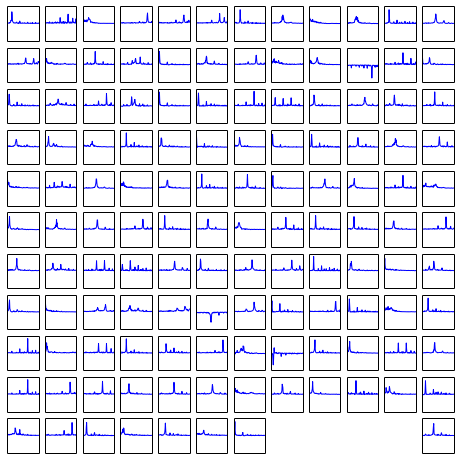
\includegraphics[width=9cm]{img/dictionary}
	\caption[]{$m=128$ atoms of a learned dictionary of spectrograms.}
	\label{fig:dictionary}
\end{figure}

\paragraph{Learned dictionary.}
\figref{dictionary} depicts a learned dictionary. Although the atoms are not easily interpretable, single notes seem to appear here and there. \cite{lecun2010PSD} showed that dictionaries trained on individual octaves did discover harmonics, chords and harmonies without any prior about music theory.

\begin{figure}[ht]
	\centering
	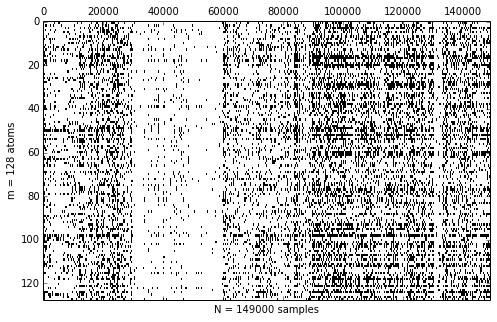
\includegraphics[width=\textwidth]{img/sparse_representations}
	\caption[]{A learned sparse representation of spectrograms.}
	\label{fig:sparse_representations}
\end{figure}

\paragraph{Sparse representations.}
\figref{sparse_representations} shows the representations inferred by \eqnref{model} after convergence. With only 19.8\% of non-zero coefficients, the learned representations are indeed sparse.

\begin{figure}[ht]
	\centering
	\begin{subfigure}[b]{0.9\textwidth}
		\centering
		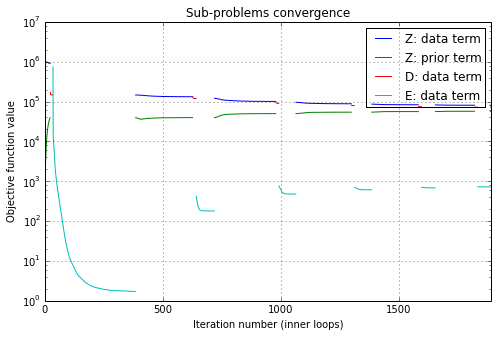
\includegraphics[height=6cm]{img/sub_problems}
		\caption{Sub-problem objectives $f_2(\Z)$, $f_1(\Z)$, $f_2(\D)$ and $f_2(\E)$ evaluated at each inner iteration.}
	\end{subfigure}
	\\
	\begin{subfigure}[b]{0.9\textwidth}
		\centering
		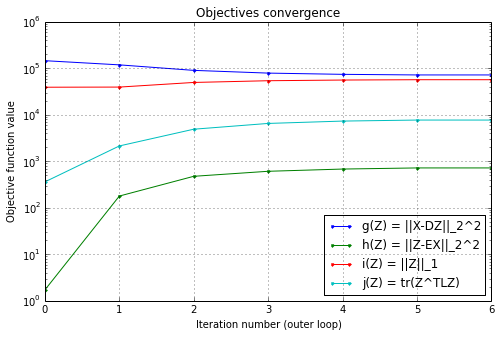
\includegraphics[height=6cm]{img/sub_objectives}
		\caption{Sub-objectives $\fd$, $\fe$, $\fz$ and $\fg$ evaluated at each outer iteration.}
	\end{subfigure}
	\\
	\begin{subfigure}[b]{0.9\textwidth}
		\centering
		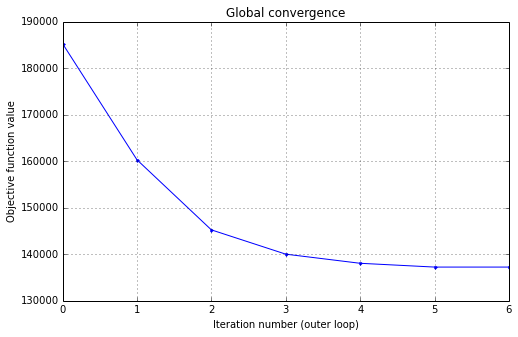
\includegraphics[height=6cm]{img/objective}
		\caption{Global objective $\fd + \fe + \fz + \fg$ evaluated at each outer iteration.}
	\end{subfigure}
	\caption[]{Example of a typical convergence of the algorithm.}
	\label{fig:convergence}
\end{figure}

\paragraph{Convergence.}

While the optimization always end in a different local minimum (\chapref{optimization}), a pretty stable convergence behavior has been observed in all the experiments. \figref{convergence} shows the evolution of the various objectives in a typical convergence of the algorithm.

%The encoder fidelity sub-objective is 2 orders of magnitude lower than the other sub-objectives, which suggests that the addition of the encoder does not alter the features extracted via the complete scheme defined by \eqnref{model}.

%\section{Descriptive features vectors}
% Show aggregated features vectors for some genres.
% How is it qualitatively more discriminative than the spectrogram ?

%\section{Hyper-parameters tuning}
% Test matrix for hyper-parameters on smaller problem (i.e. less frames).
% For ld, le, lg, m
% Numerical parameters: Nouter (enough when no more inner), rtol
% Graph parameters: K, Csigma, kernel?, metric
% Classification: C, Nvectors
% Pre-processing: na=1024, ns=96

% Overcompleteness, defined by the hyper-parameter $m$, must be evaluated by considering the number of code units and the effective dimensionality of the input as given by \gls{PCA}.

%\section{Classification accuracy}
% On the whole dataset, not very good in comparison with others.
% Measured via 10-fold cross-validation
% How classification is improved by features learning, introducing the encoder / graph.
% Comparison with other techniques.
% State what the hyper-parameters are.

%\section{Sparse representations}
% The extracted representations are indeed sparse.

%\section{Scarce training set}
% Il faut juste garder à l'esprit que le graphe (et le dictionnaire) est appris sur le dataset complet. Ça peut cependant être utile si on a beaucoup de données à disposition mais que les labels coûtent chers.

\section{Classification performance}
% Final experiement: baseline, graph-less, graph vs noise level
% Robustness to noisy data

\tabref{classification_accuracy} shows the classification accuracy when using \gls{CQT} spectrograms (the baseline), extracted features with $\lambda_g=0$ (sparse auto-encoder) and $\lambda_g=100$ (structured auto-encoder). The other hyper-parameters are set to $\lambda_z=1$, $\lambda_d=10$ and $\lambda_e=0$.

The first conclusion to draw from this experiment is that the representation extracted from the spectrograms by the structured auto-encoder defined in \partref{algorithm} is indeed more discriminative than the spectrograms themselves in a classification task.

The second conclusion we can draw is that the addition of the smooth prior on the data manifold (\secref{manifold_learning}) always lead to an improved accuracy.

Finally, the sparse and structured representations are robust with respect to noisy data. While a sparse auto-encoder ($\lambda_g=0$) performs even worse than the baseline, our structured auto-encoder ($\lambda_g=100$) out-performs the baseline by 7\%.

\begin {table}[H]
\begin{center}
	\begin{tabular}{|l|c|c|c|c|}
		\hline
		Noise level (standard deviation)  & 0.00 & 0.10 & 0.20 \\
		\hline
		Accuracy (baseline) [\%]          & 69.7 & 58.7 & 46.9 \\
		Accuracy ($\lambda_g=0$) [\%]     & 75.9 & 57.1 & 42.6 \\
		Accuracy ($\lambda_g=100$) [\%]   & 78.0 & 65.9 & 51.6 \\
		\hline
	\end{tabular}
	\caption{Classification accuracies on a subset of GTZAN: $N_{genres} = 5$ genres, $N_{clips} = 100$ clips per genre and $N_{frames} = 149$ frames per clip.}
	\label{tab:classification_accuracy}
\end{center}
\end{table}

%The second experiment shows that structured representations are robust to noise.

%M: However in the noiseless environment the addition of the graph is not significant.
%X: oui, mais tu ne dois pas oublier que tu fais du *transductive* learning, c'est a dire tu apprends les features en utilisant training + TEST data. C'est pour cela que tu n'as pas une amelioration significative. Si on faisait du *supervised* learning, c'est a dire on utilise seulement les TRAINING data, alors ce probleme est bcp plus challenging que le transductive probleme, et la je pense que nos resultats avec graph seraient bien meilleures! C'est un commentaire que je te conseille d'ajouter a ton resultat pour le mettre en perspective. Aussi la premiere chose a faire apres le PDM est de faire du *supervised* learning avec graph et le comparer avec no graph, je pense que l'on aura des (bonnes) surprises!

\section{Discussion}
% Is the model appropriate for the problem ?

%While our results are far from the state-of-the-art in \gls{MGR} on GTZAN,
Our experiments demonstrated the usefulness of an important property of the proposed model: the conservation of the structure in the data via graph regularization. When compared to a sparse auto-encoder, it always leads to a better accuracy, especially in a noisy scenario, when the structure is the most helpful.
%hich allows the system to be robust to noisy data.

We experimentally confirmed two assumptions of our model (\secref{assumptions}): the learned representations are sparse (\figref{sparse_representations}) and structured.
%we made the point that our model is useful and that we shall continue to research on it.

Higher classification accuracies are probably achievable by fine-tuning the hyper-parameters and introducing adding further complexity; e.g. by applying a \gls{LCN} to the \gls{CQT} spectrograms or working on individual octaves, two techniques used by \cite{lecun2011PSDaudio}. We may even further improve the performance of our model by creating better graphs, i.e. graphs more suited to the problem at hand, for example by tuning the construction hyper-parameters.